\chapter{Evaluation\label{cha:evaluation}}

In this chapter the Orchestrator introduced in chapter \ref{cha:orchestrator} is tested and evaluated. For this purpose an object detection application is used, which should be deployed to a given test infrastructure containing several devices. In the first experiment the nodes join and leave the network one after the other. In the second experiment all nodes are online, but the network connection quality is manipulated. For both experiments it is examined which decisions the Orchestrator makes and what effect this decision has on the total latency of the application.







\section{Experimental setup}

\subsection{Infrastructure\label{sec:eval-infrastructure}}

\begin{figure}[htb]
    \centering
    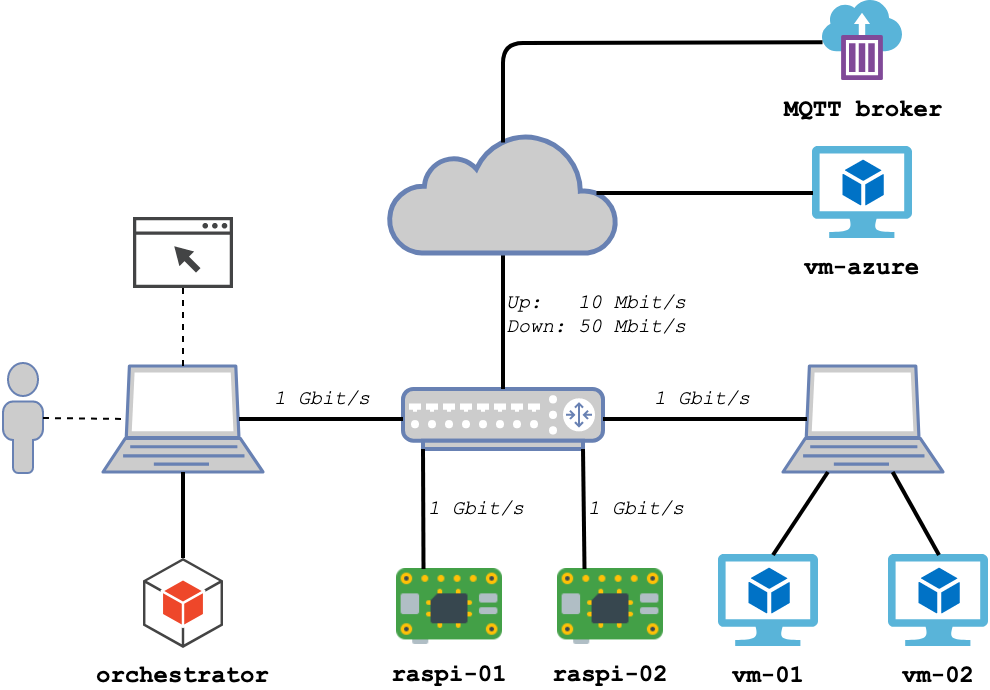
\includegraphics[width=0.85\textwidth]{evaluation-infrastructure}
    \caption{Test infrastructure for evaluation}
    \label{fig:evaluation-infrastructure}
\end{figure}

The test bed consists of the five nodes shown in figure \ref{fig:evaluation-infrastructure}. The hardware characteristics of the devices are shown in table \ref{tab:evaluation-devices}. The three virtual machines run Debian 10, the two Raspberry Pis run Raspbian 10. All nodes have \texttt{Docker version 19.03.2} installed. Another device on the local network runs the Orchestrator and a web browser which is used to access the \textit{Object Detection Web Application}. Communication between the nodes and the Orchestrator is done via an MQTT broker running in the Azure Cloud.

\begin{table}[htb]
    \centering
    \begin{tabular}{|l|l|l|l|l|l|}
    \hline
        \textbf{Node} & \textbf{Device Type} & \textbf{CPU} & \textbf{RAM} \\
         \hline
         \texttt{raspi-01} & Raspberry Pi 3B+ & ARM Cortex-A53 1.4 GHz, 4 cores & 1 GB\\
         \hline
         \texttt{raspi-02} & Raspberry Pi 4B & ARM Cortex-A72 1.5 GHz, 4 cores & 4 GB\\
         \hline
         \texttt{vm-01} & Hyper-V VM & Intel i7-8550U 1.8 GHz, 2 vCPUs & 2 GB\\
         \hline
         \texttt{vm-02} & Hyper-V VM & Intel i7-8550U 1.8 GHz, 4 vCPUs & 4 GB\\
         \hline
         \texttt{vm-azure} & Azure VM \texttt{F4s\_v2} & Intel Xeon 2.7 GHz, 4 vCPUs & 8 GB\\
         \hline
    \end{tabular}
    \caption{Hardware characteristics of test devices used for evaluation}
    \label{tab:evaluation-devices}
\end{table}

\subsection{Application\label{sec:eval-application}}

\begin{figure}[htb]
    \centering
    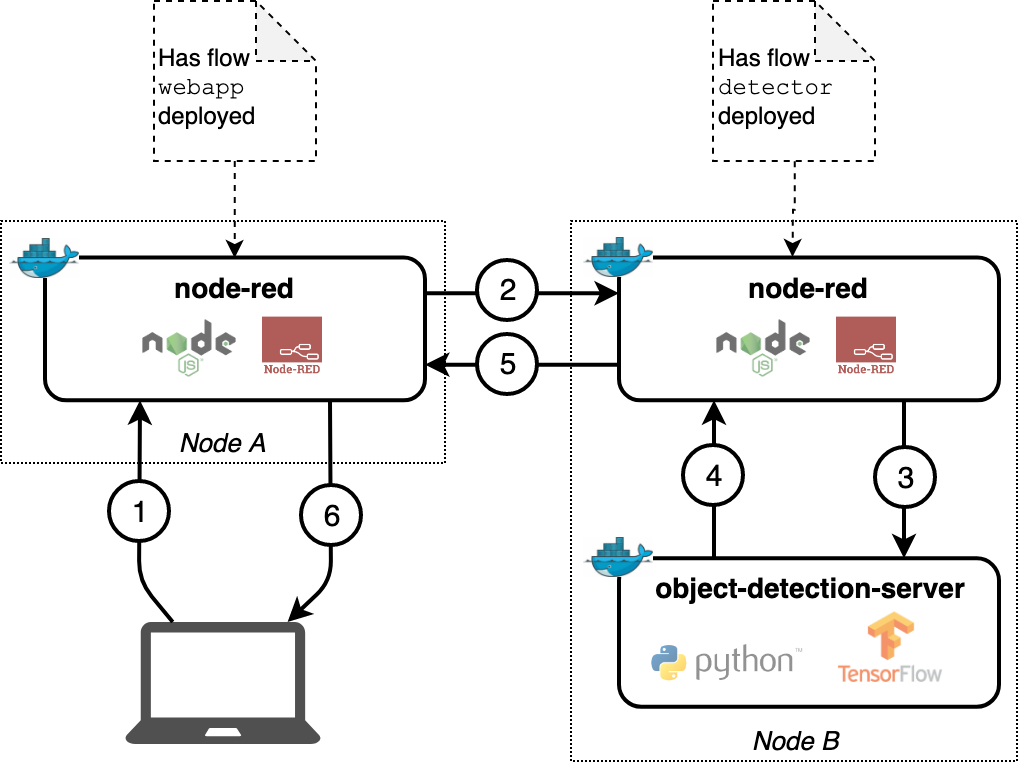
\includegraphics[width=0.85\textwidth]{evaluation-application}
    \caption{System architecture of Object Detection Web Application}
    \label{fig:evaluation-object-detection-application}
\end{figure}

The \textit{Object Detection Web Application} consists of the two modules \texttt{webapp} and \texttt{detector} as illustrated in figure \ref{fig:evaluation-object-detection-application}. A screenshot of the web application is shown in figure \ref{fig:object-detection-webapp-screenshot}.\\

In the first step, a user sends an image for object detection to the \texttt{webapp} module which is deployed as a Node-RED flow on \texttt{Node A}. This module should always be deployed on the same node and not be moved so that the web application is always available at the same address. The user calls the web application from that fixed node and he does not care which node actually executes the object detection task. The module \texttt{webapp} forwards the image to the module \texttt{detector} for object detection which is deployed on another node (\texttt{Node B}). This node can vary and is chosen by the Orchestrator. If a new node is selected by the Orchestrator, then the flow \texttt{webapp} on \texttt{Node A} will be updated so that subsequent requests are forwarded to the new node.\\

The object detection engine can not be executed as a regular Node-RED flow since Node-RED handles JavaScript functions only and the engine requires Python. Even if Node-RED could execute Python code (there are extensions enabling this) the execution of the object detection engine in Node-RED would not be efficient because the engine would have to be initialized every time a new object detection request arrives. However, the engine has a certain initialization time to load the detection graph. Therefore it is more efficient to initialize the engine only once at the beginning so that the following object detection tasks can be executed without additional initialization time. Because Node-RED can not initialize and hold Python objects, a separate docker container is used for this purpose. The flow \texttt{detector} sends an HTTP request containing the undetected image to the \texttt{object-detection-server} running on the same node. The server responds with the detected image which the \texttt{detector} then sends back to the \texttt{webapp} module.

The following three constraints are defined for the experiment:
\begin{enumerate}
    \item The flow \texttt{webapp} must be deployed on \texttt{raspi-01} because this is the only node known to the user
    \item The flow \texttt{detector} needs an \texttt{object-detection-server} docker container running on the same node which is the case for all nodes except for \texttt{raspi-01}
    \item The detected image must be available within 5 seconds
\end{enumerate}








\section{Preparing the Orchestrator\label{sec:eval-preparing-the-orchestrator}}

For evaluating the Orchestrator we need nodes with different CPU performance(s?).
However, one vCPU in \texttt{vm-01} is equally fast as in \texttt{vm-02} because they both run on the same host.
Since the object detection engine uses only one core, the execution time on these two nodes is approximately the same, although \texttt{vm-01} has two cores and \texttt{vm-02} has four cores. For this reason, the docker containers on \texttt{vm-01} run with the additional option \texttt{---cpus="0.5"} which limits the available CPU resources a container can use to a half vCPU.

\subsection{Possible deployment strategies and their respective latencies\label{sec:eval-possible-deployments}}
To find the real execution times of all possible deployment strategies, the application was deployed to the infrastructure without using the Orchestrator.
The module \texttt{webapp} was always deployed on node \texttt{raspi-01} while the module \texttt{detector} was switched through the remaining nodes.
The object detection application was executed 10 times on each deployment strategy by using a 1,383 KB sized image.
The mean values for \textit{total latency}, \textit{processing time} and \textit{transfer time} were calculated thereafter. These are compared in figure \ref{fig:evaluation-total-latency-without-orchestrator}.

\begin{figure}[h!]
    \centering
    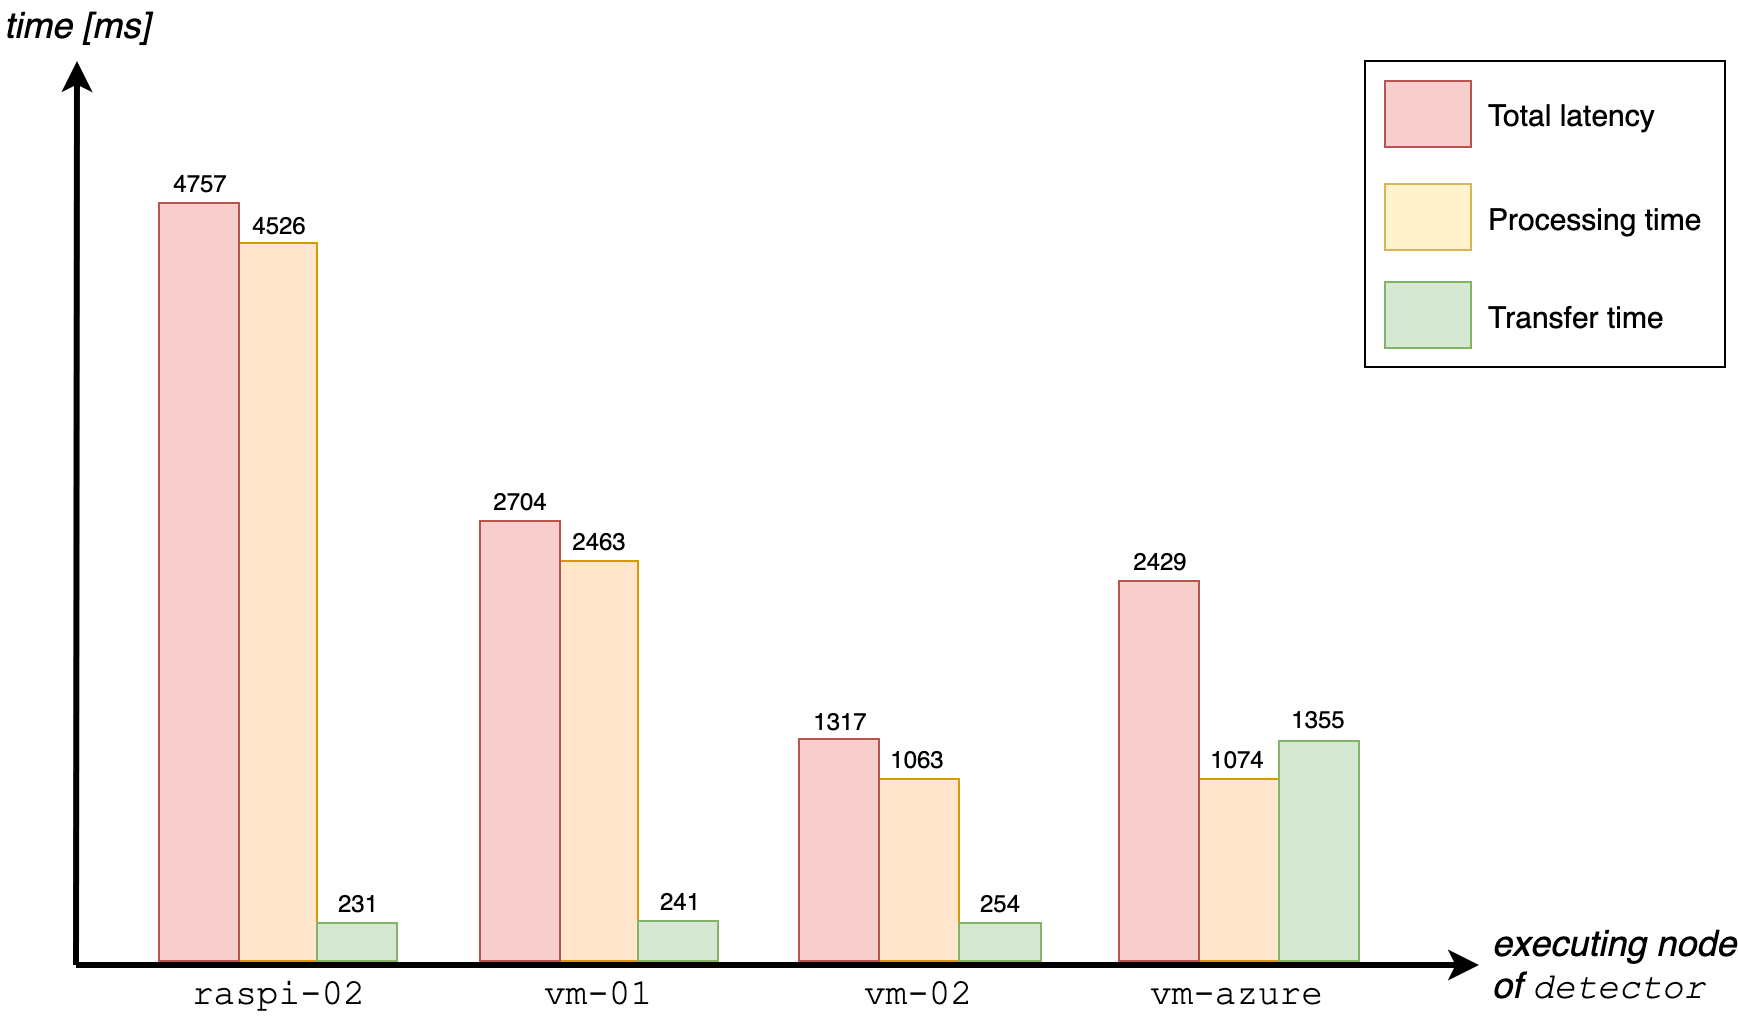
\includegraphics[width=1.0\textwidth]{evaluation-total-latency-without-orchestrator}
    \caption{Total latencies, processing and transfer times of the object detection application regarding the placement of module \texttt{detector}}
    \label{fig:evaluation-total-latency-without-orchestrator}
\end{figure}

Based on the measurement results, a prioritization of all possible deployments was created where deployments with a lower latency were preferred (see table \ref{tab:deployment-strategies-prios}).
\begin{table}[h!tb]
    \centering
    \begin{tabular}{|l|l|l|l|l|l|}
    \hline
        \textbf{Priority} & \textbf{Placement of \texttt{webapp}} & \textbf{Placement of \texttt{detector}} & \textbf{Latency} \\
         \hline
         \texttt{1} & \texttt{raspi-01} & \texttt{vm-02} & 1,317 ms\\
         \hline
         \texttt{2} & \texttt{raspi-01} & \texttt{vm-azure} & 2,429 ms\\
         \hline
         \texttt{3} & \texttt{raspi-01} & \texttt{vm-01} & 2,704 ms\\
         \hline
         \texttt{4} & \texttt{raspi-01} & \texttt{raspi-02} & 4,757 ms\\
         \hline
    \end{tabular}
    \caption{Possible deployment strategies \textcolor{red}{\textbf{for (of?)}} object detection application}
    \label{tab:deployment-strategies-prios}
\end{table}

\subsection{Defining the Application\label{sec:eval-defining-application}}

Although the Orchestrator handles the infrastructure dynamically, an application must be defined. Therefore, an instance of \texttt{Application} is created during the initialization of the Orchestrator.
It contains all modules, loops and messages of the object detection application described in section \ref{sec:eval-application}.

\subsubsection*{Setting required RAM and disk storage}
The fields \texttt{requiredRam} and \texttt{requiredStorage} of the two modules \texttt{webapp} and \texttt{detector} are set to \texttt{0} because both Node-RED flows are relatively small and thus consume neither significant RAM nor storage.
Although the \texttt{object-detection-server} container requires 1GB RAM, this memory is not allocated/released by deploying/removing the flow to/from Node-RED because the container runs even if the Node-RED flow is not deployed on a node.
Furthermore, the container does not require any additional disk storage while running the engine.

\subsubsection*{Setting required hardware modules}
The field \texttt{requiredHardwareModules} of the module \texttt{webapp} contains one string: \texttt{"CAMERA"}.
The \texttt{node-red} docker container on \texttt{raspi-01} is started with the additional option \texttt{-e CONNECTED\_HARDWARE=["CAMERA"]} so that \texttt{webapp} can only be deployed \textcolor{red}{\textbf{on (to?)}} \texttt{raspi-01}. The same approach is used for the module \texttt{detector}, but here the string \texttt{"OD-DOCKER-CONTAINER"} is used and passed to the docker container on the remaining nodes instead.

\subsubsection*{Setting required instructions}
The field \texttt{requiredMi} of the module \texttt{webapp} is set to \texttt{0} because the Node-RED flow simply forwards messages and therefore does not require any significant CPU power.
However, CPU resources consumed by the module \texttt{detector} are substantial.
Since the Orchestrator uses a CPU score instead of MIPS, the value for \texttt{requiredMi} has to be calculated using the formula introduced in section \ref{sec:benchmark-cpu}.
Values for \textit{CPU score} and \textit{execution time} are taken from \texttt{vm-02}, which are \textit{11661} and \textit{1317 ms}, respectively.
Therefore:
\[\textrm{\texttt{requiredMi\textsubscript{detector}}} = \textrm{CPU score} \boldsymbol{\cdot} \frac{\textrm{execution time [ms]}}{1,000 \textrm{ [ms]}} = 11,661 \boldsymbol{\cdot} \frac{1,317}{1,000} = 15,357\]

\subsubsection*{Setting the loop and messages}
The application has exactly one loop (instance of \texttt{AppLoop}) where the field \texttt{modules} is populated with a list containing three elements in the following order:
\texttt{"webapp"}, \texttt{"detector"}, \texttt{"webapp"}.
The field \texttt{maxLatency} is set to \texttt{5000}.

Furthermore, the application contains two messages (instaces of \texttt{AppMessage}).
The first one contains the original image, which in this case has a file size of 1,383 KB. Therefore, the fields \texttt{contentType} and \texttt{dataPerMessage} are set to \texttt{"IMAGE\_UNDETECTED"} and  \texttt{1383}, respectively. This is the input message to the module \texttt{detector}.
The second message contains the detected image, which has a file size of 142 KB. Therefore, the fields are set to \texttt{"IMAGE\_DETECTED"} and \texttt{142}, respectively. This is the output message of the module \texttt{detector}.









\section{Experiment 1: Consistent network quality\label{sec:eval-exp-1}}

In this experiment, the nodes are started in the following order:
\begin{enumerate}
    \item \texttt{raspi-01}
    \item \texttt{raspi-02}
    \item \texttt{vm-01}
    \item \texttt{vm-azure}
    \item \texttt{vm-02}
\end{enumerate}
This order allows to deploy the deployment strategy with the lowest priority in step two, while with each following step a strategy of higher priority is possible (see table \ref{tab:deployment-strategies-prios}).

\subsection{Expected decisions}
In the first step the Orchestrator shouldn't find a valid deployment because here only \texttt{raspi-01} is online which is not able to execute the module \texttt{detector}.
It is expected that the Orchestrator deploys the module \texttt{webapp} to \texttt{raspi-01} and \texttt{detector} to \texttt{raspi-02} in the second step and then moves the \texttt{detector} to \texttt{vm-01}, \texttt{vm-azure} and \texttt{vm-02} in the subsequent steps, while \texttt{webapp} remains on \texttt{raspi-01}.

\subsection{Actual decisions}

The Orchestrators decisions are depicted in figure \ref{fig:evaluation-exp1-results}. As we can see, the Orchestrator behaved slightly different than expected. The \texttt{detector} was expected to be deployed to \texttt{raspi-02} in the second step. However, this did not happen. Instead, no possible deployment was found. In steps 1, 3, 4 and 5, however, the Orchestrator made the correct decisions as expected and latency is continuously minimized from step 3 onwards.

\begin{figure}[htb]
    \centering
    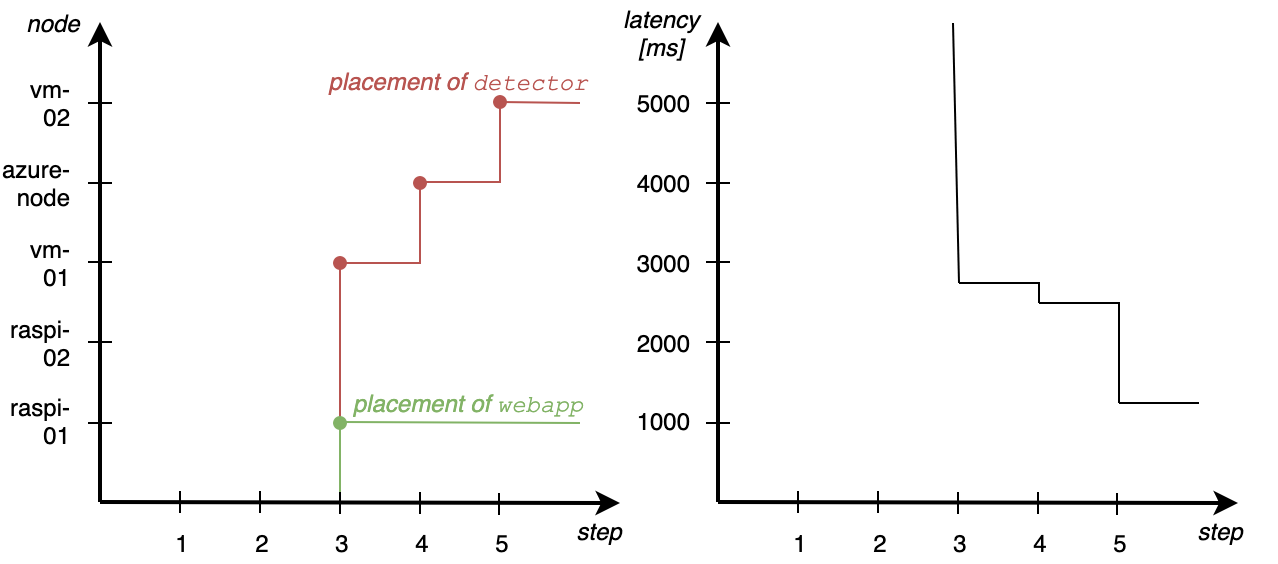
\includegraphics[width=1.0\textwidth]{evaluation-exp1-result}
    \caption{Result of Experiment 1: Orchestrators decisions and their impact on total latency}
    \label{fig:evaluation-exp1-results}
\end{figure}

Moreover, it was examined how the Orchestrator behaves when a node leaves the network.
If a node that has \textit{no} module deployed leaves the network, the Orchestrator detects this and removes it from the infrastructure. The deployment strategy remains unchanged as it should be.
If a node that \textit{has} a module deployed leaves the network, the Orchestrator detects this and removes it from the infrastructure first before it then finds and applies the next best possible deployment strategy (next best deployment strategy is the one of highest priority in the updated infrastructure).
This complies with the desired behaviour.

\subsection{Investigation of the Orchestrators incorrect decision\label{sec:eval-investigation-cpu}}

The reason for the wrong decision in step two is that the execution time of module \texttt{detector} on node \texttt{raspi-02} calculated by the Orchestrator is incorrect.
The field \texttt{cpuMips} of the \texttt{FogNode} object representing this node has the value 973.
This value is the CPU score returned by the \texttt{benchmark\_cpu} command which the Orchestrator executed on the node after the first heartbeat has been received (see section \ref{sec:handling-new-fog-nodes} and \ref{sec:benchmark-cpu} in particular).
To calculate the execution time of module \textit{M} on node \textit{N}, the Orchestrator uses \texttt{cpuMips} of N and \texttt{requiredMi} of M.
While preparing the Orchestrator in section \ref{sec:eval-preparing-the-orchestrator}, we set \texttt{requiredMi\textsubscript{detector}} to 15,357. Thus, the execution time is calculated as follows:

\[\textrm{execution time [ms]} = \frac{\textrm{\texttt{requiredMi}}}{\textrm{\texttt{cpuMips}}}\ \boldsymbol{\cdot} 1,000 = \frac{15,357}{973}\ \boldsymbol{\cdot} 1,000 = 15,783 \textrm{ [ms]}\]

The calculated execution time is approximately 3.5 times greater than actual execution time of 4,526 milliseconds (see figure \ref{fig:evaluation-total-latency-without-orchestrator}).
Furthermore, it is greater than 5,000 milliseconds, which is the \texttt{maxLatency} of the opject detection loop. 
Therefore, the Orchestrator finds no valid deployment strategy.

The \texttt{benchmark\_cpu} command internally uses the CPU benchmarking tool \texttt{sysbench} which searches for all prime numbers between 1 and a certain upper limit (2000 in this case) and returns the time needed to execute this task.
Apparently, this time cannot be used to deduce the execution time of other types of tasks like object detection.
To further investigate this, the simple JavaScript function shown in listing \ref{lst:simple-javascript-function} was executed in Node-RED on \texttt{raspi-02} and \texttt{vm-02}.

\begin{lstlisting}[language=JavaScript,numbers=none,caption={JavaScript function which calculates a simple mathematical problem while measuring the execution time},label=lst:simple-javascript-function]
const timeStart = new Date();
let result = 0;
for (let i=0; i < Math.pow(10,7); i++) {
    result = result + i;
}
const timeEnd = new Date();
const time = timeEnd - timeStart;
\end{lstlisting}

The field \texttt{time} of that function contains the execution time in milliseconds which is approximately 2,500 on \texttt{vm-02} and 7,500 on \texttt{raspi-02}, respectively. 
Thus, the execution of the function is about \textit{3 times faster} on \texttt{vm-02} than on \texttt{raspi-02}, even though the CPU score of \texttt{vm-02} (11,848) is about \textit{12 times greater} than the score of \texttt{raspi-02} (973).
What's more, the object detection task takes about 1,063 milliseconds on \texttt{vm-02} and 4,757 milliseconds on \texttt{raspi-02}, which is a \textit{4,2-fold difference} (see figure \ref{fig:evaluation-total-latency-without-orchestrator}). A correlation can therefore not be recognized.

However, there might be a correlation between CPUs that have the same architecture, but this is not the case either:
Executing the function shown in listing \ref{lst:simple-javascript-function} takes about 17,800 milliseconds on \texttt{raspi-01}, which is \textit{2.37 times slower} than on \texttt{raspi-02}, although the CPU score of \texttt{raspi-01} (612) is only \textit{1.59 times smaller} than on \texttt{raspi-02}. Both nodes own a CPU of type \texttt{arm}.\\

In conclusion, the execution time of a given task cannot be used as the basis to compare CPU performance of different devices.
There seem to be a number of relevant factors affecting the execution time of a task, but this goes beyond the scope of this work.


\section{Experiment 2: Volatile network conditions}

TODO

\section{Discussion}

TODO

- CPU: Intel -> gut vergleichbar; ARM -> nicht gut vergleichbar
alternative methode: test ausführung von modules und sich die zeit merken

problem: input size --> auch hier wären erfahrungswerte besser

Problem: webapp hat zwei input und zwei output types

problem: netzwerkmessungen bei vielen nodes